\documentclass[tikz,border=2mm]{standalone}
\usetikzlibrary{positioning,arrows.meta,calc,decorations.pathreplacing,shapes.geometric,fit}
\definecolor{flowblue}{HTML}{DAE8FC}\definecolor{flowblueline}{HTML}{6C8EBF}
\definecolor{flowgreen}{HTML}{D5E8D4}\definecolor{flowgreenline}{HTML}{82B366}
\definecolor{flowpurple}{HTML}{E1D5E7}\definecolor{flowpurpleline}{HTML}{9673A6}
\definecolor{flowgrey}{HTML}{F5F5F5}\definecolor{flowgreyline}{HTML}{999999}
\begin{document}
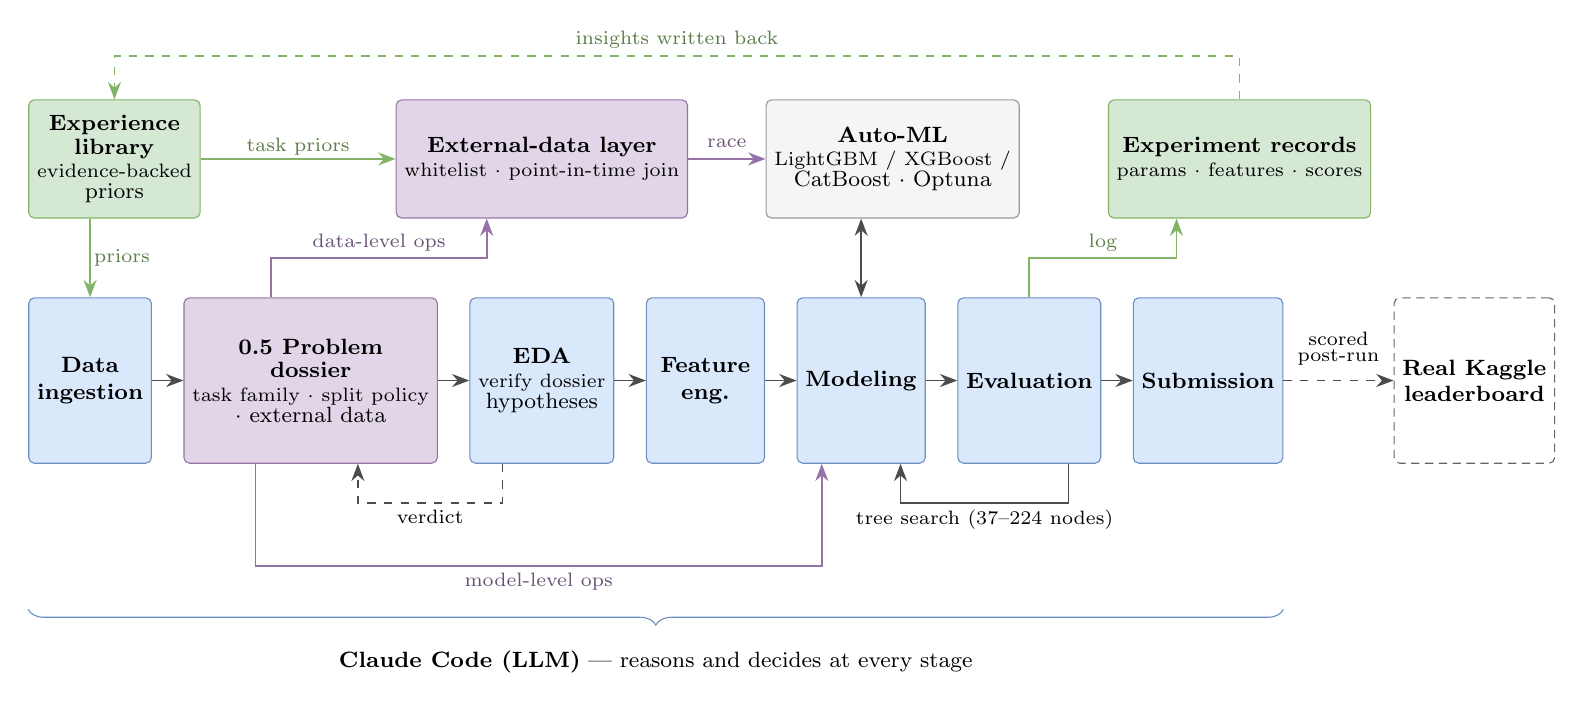
\begin{tikzpicture}[
  font=\footnotesize,
  stage/.style={draw=flowblueline, rounded corners=2pt, align=center, inner sep=3pt,
                fill=flowblue, minimum height=21mm, minimum width=15mm},
  inj/.style={stage, fill=flowpurple, draw=flowpurpleline},
  supp/.style={draw=flowgreenline, rounded corners=2pt, align=center, inner sep=3pt,
               fill=flowgreen, minimum height=15mm},
  injbox/.style={supp, fill=flowpurple, draw=flowpurpleline},
  toolbox/.style={supp, fill=flowgrey, draw=flowgreyline},
  arr/.style={-{Stealth[length=2.2mm]}, semithick, black!70},
  parr/.style={arr, flowpurpleline},
  garr/.style={arr, flowgreenline},
  darr/.style={arr, dashed},
  lab/.style={font=\scriptsize, align=center, inner sep=1.2pt},
  glab/.style={lab, text=flowgreenline!70!black},
  plab/.style={lab, text=flowpurpleline!70!black}
]
% ================= main pipeline: one left-to-right spine =================
\node[stage] (s1) at (0,0) {\textbf{Data}\\\textbf{ingestion}};
\node[inj, right=4mm of s1] (s05)
  {\textbf{0.5 Problem}\\[-1pt]\textbf{dossier}\\[-1pt]
   \scriptsize task family $\cdot$ split policy\\[-2pt]$\cdot$ external data};
\node[stage, right=4mm of s05] (s2)
  {\textbf{EDA}\\[-1pt]\scriptsize verify dossier\\[-2pt]hypotheses};
\node[stage, right=4mm of s2]  (s3) {\textbf{Feature}\\\textbf{eng.}};
\node[stage, right=4mm of s3]  (s4) {\textbf{Modeling}};
\node[stage, right=4mm of s4]  (s5) {\textbf{Evaluation}};
\node[stage, right=4mm of s5]  (s6) {\textbf{Submission}};
\node[stage, densely dashed, fill=white, draw=black!60, right=14mm of s6] (lb)
  {\textbf{Real Kaggle}\\\textbf{leaderboard}};
\foreach \a/\b in {s1/s05, s05/s2, s2/s3, s3/s4, s4/s5, s5/s6}{\draw[arr] (\a) -- (\b);}
% pipeline endpoint: the real leaderboard
\draw[darr] (s6) -- (lb);
\node[lab, above=1.4mm] at ($(s6.east)!0.5!(lb.west)$) {scored\\[-2pt]post-run};
% ================= rail row above the spine =================
\node[supp,    anchor=south west] (lib)   at ([yshift=10mm]s1.north west)
  {\textbf{Experience}\\[-1pt]\textbf{library}\\[-1pt]
   \scriptsize evidence-backed\\[-2pt]priors};
\node[injbox,  anchor=south]      (ext)   at ([yshift=10mm]s2.north)
  {\textbf{External-data layer}\\[-1pt]
   \scriptsize whitelist $\cdot$ point-in-time join};
\node[toolbox, anchor=south]      (tools) at ([xshift=4mm,yshift=10mm]s4.north)
  {\textbf{Auto-ML}\\[-1pt]\scriptsize LightGBM / XGBoost /\\[-2pt]CatBoost $\cdot$ Optuna};
\node[supp,    anchor=south]      (rec)   at ([xshift=4mm,yshift=10mm]s6.north)
  {\textbf{Experiment records}\\[-1pt]
   \scriptsize params $\cdot$ features $\cdot$ scores};
% ----- rail to rail (top band) -----
\draw[garr] (lib.east) -- node[glab, above]{task priors} (ext.west);
\draw[parr] (ext.east) -- node[plab, above=0.9mm]{race} (tools.west);
% ----- rail <-> spine connectors -----
\draw[garr] (lib.south -| s1.north) -- node[glab, right]{priors} (s1.north);
\draw[arr, {Stealth[length=2.2mm]}-{Stealth[length=2.2mm]}] (tools.south -| s4.north) -- (s4.north);
% dossier -> external-data layer (data-level operators)
\coordinate (dlA) at ([xshift=-5mm,yshift=5mm]s05.north);
\coordinate (dlB) at ([xshift=-7mm]ext.south);
\draw[parr] ([xshift=-5mm]s05.north) -- (dlA) -| (dlB);
\node[plab, above=0.4mm] at ($(dlA)!0.5!(dlB |- dlA)$) {data-level ops};
% evaluation -> experiment records
\coordinate (lgA) at ([yshift=5mm]s5.north);
\coordinate (lgB) at ([xshift=-8mm]rec.south);
\draw[garr] (s5.north) -- (lgA) -| (lgB);
\node[glab, above=0.4mm] at ($(lgA)!0.5!(lgB |- lgA)$) {log};
% ----- dashed write-back, along the very top -----
\coordinate (wbA) at ([yshift=5.5mm]rec.north);
\coordinate (wbB) at (lib.north);
\draw[darr, flowgreenline] (rec.north) -- (wbA) -| (wbB);
\node[glab, above=0.5mm] at ($(wbA)!0.5!(wbB |- wbA)$) {insights written back};
% ================= feedback lanes below the spine =================
% EDA verdict back to the dossier
\coordinate (vdA) at ([xshift=-5mm,yshift=-5mm]s2.south);
\coordinate (vdB) at ([xshift=6mm]s05.south);
\draw[darr] ([xshift=-5mm]s2.south) -- (vdA) -| (vdB);
\node[lab, below=0.4mm] at ($(vdA)!0.5!(vdB |- vdA)$) {verdict};
% tree-search loop: Evaluation -> Modeling
\coordinate (tsA) at ([xshift=5mm,yshift=-5mm]s5.south);
\coordinate (tsB) at ([xshift=5mm]s4.south);
\draw[arr] ([xshift=5mm]s5.south) -- (tsA) -| (tsB);
\node[lab, below=0.4mm] at ($(tsA)!0.5!(tsB |- tsA)$) {tree search (37--224 nodes)};
% model-level operators: dossier seeds the search directly
\coordinate (mlA) at ([xshift=-7mm,yshift=-13mm]s05.south);
\coordinate (mlB) at ([xshift=-5mm]s4.south);
\draw[parr] ([xshift=-7mm]s05.south) -- (mlA) -| (mlB);
\node[plab, below=0.4mm] at ($(mlA)!0.5!(mlB |- mlA)$) {model-level ops};
% ================= LLM annotation: horizontal brace under the stages =====
\draw[decorate, decoration={brace, amplitude=2mm}, flowblueline]
  ([yshift=-18.5mm]s6.south east) -- ([yshift=-18.5mm]s1.south west)
  node[midway, yshift=-4mm, anchor=north, black]
  {\textbf{Claude Code (LLM)} --- reasons and decides at every stage};
\end{tikzpicture}
\end{document}
